\documentclass[a4paper,10pt]{article}
\usepackage{graphicx}
\usepackage[pdfborder={0 0 0}]{hyperref}
\title{ Student Project 2017 \\ CalTech101 Image Classification}
\author{David Schulte, Hannes Martinke, Martin Zettwitz}

\begin{document}
\maketitle

\section{Introduction}
\subsection{Problem}
The classification of arbitrary pictures is an actual very hard task for image analysts, because the machine learning methods are difficult to use with the high number of pixel features in an image.
The task of the project is to classify the \emph{CalTech 101} dataset by using different feature selection and classifing approaches. 
101 different image categories the data set contains and the aim is a valdiation accuracy of 10~\% with an 10-Fold cross validation.
\subsection{Programming Environment}
Our classification approach is implemented in C++ with the including of \emph{Opencv} and \emph{dlib}.
\emph{Opencv} and \emph{dlib} are open source libraries for computer vision and machine learning tasks. 
Out first approaches were a complete implementation in \emph{Opencv}, but because of some missing algorithm for the classification step in the library, we add the \emph{dlib} and combine both libraries in the implementation.
The workflow of our procedure is illustrated in \autoref{fig:workflow}. and consists the following 4 steps: image preprocessing, features, classifier, validation.
These steps will be explained in the next sections.

\begin{figure}[ht]
\centering
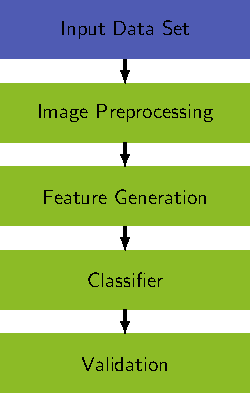
\includegraphics[scale=1]{images/Workflow.pdf}
\caption{Our Worklow for the image classification. We organized the input data sets and prepare each image for the subsequent feature generation.
This feature are integrated in the classifier and the validation is performed in the next step to evaluate the classification results.}
\label{fig:workflow}
\end{figure}

\section{Preprocessing}
\label{sec:preprocessing}
Several images in the \emph{CalTech 101} dataset exist with different image sizes. 
This follows in different feature vector lengths in the feature generation.
To avoid this and to standardizes the vector length we resized each image in the data set to 64x64.
An additional reason for the resizing is the duration time of the complete algorithm. 
We tried to get a good trade-off between accuracy and duration time and this is a good solution after analyzing several image classes.
\begin{figure}[ht]
\centering
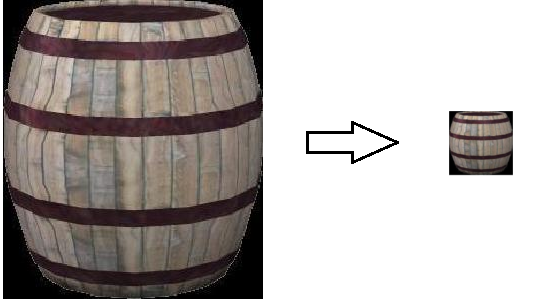
\includegraphics[scale=0.5]{images/preprocessing.png}
\caption{Illustration of the image resampling with an example image of a barrel.}
\label{fig:resize}
\end{figure}

\section{Features}
\subsection{Feature Generation}

In this section for each resampled images the features will be calculated by different approaches.
We used the Histogram-of-Gradient~(HOG) features and the other feature generation technique is the detection of Local Binary Patterns~(LBP) features.
\paragraph{Histogram-of-Gradients}

The first feature generation technique we used is the \textbf{HOG descriptor}.
This is a detector, which calculates the oriented gradients in the image for predefined cells. 
This cell size in combination with an x- and y-padding are the parameters for this method.
Because of the input image size it is necessary to choose a cell size, which is a divider of 64. 
We tested the cell size the 16 and 8 for feature generation. We do not want a zero border padding, so the padding values are zero. 
We used the features extracting algorithm of \emph{dlib}, which calculates an 31 dimensional feature vector for each cell.
Two example images with the different parameters is shown in figure...
\paragraph{Local Binary Patterns}
??

\subsection{Feature Reduction}

The calculated features can be reduced by using for example principle component analysis(PCA) or other techniques.
In our approach an feature reduction is served by resampling the images in the preprocessing step (recall \autoref{sec:preprocessing}).
With the limitation of the pixel matrix and the using of the HOG Features the length of the feature vector is standardized for each sample.

\section{Classifier}
\paragraph{AdaBoost}
\paragraph{SVM}

\section{Training and Validation}
10 Fold

\section{Results}
Matrix + Conclusion 

\end{document}

